\section{Summary of Methods}
\subsection{TC Counts as a Function of ENSO's phase}
ENSO phase data was acquired from the NOAA Climate Prediction Center. NINO and NINO episodes were based on a threshold of +/- $1^\circ$C for the Oceanic Ni\~{n}o Index (ONI) [3 month running mean of ERSST.v3b SST anomalies in the Ni\~{n}o 3.4 region ($5^\circ$N-$5^\circ$S, $120^\circ$-$170^\circ$W)], based on centered 30-year base periods updated every 5 years. Cold and warm episodes are defined when the threshold is met for a minimum of 5 consecutive over-lapping seasons.

\begin{table}
\begin{tabular}{cccccc}
\hline
&NINO (N = 16) & Neutral (N= 36) & NINA (N = 10)\\
\hline
Mean Aug-Oct TC counts & 7.8 & 11.06 & 11.44\\
Standard deviation & 3.17 & 4.37 & 3.54\\
\hline
\end{tabular}
\caption{The mean Aug-Oct TC counts based on the phase of ENSO. NINO years we defined as years with more than $+1^\circ$C warming anomaly. NINA years were years with less than $-1^\circ$C anomaly. Neutral years were years with warming between $-1^\circ$C and $+1^\circ$C. Given the large overlap between each group we cannot reject the null hypothesis that any two quantities are equal.}
\label{ref:table_nino_vs_tc_counts}
\end{table}

\subsection{S-ENSO}
The S-ENSO index is computed by first averaging the SST anomalies over the June-October period to accurately capture ENSO's evolution prior to and during the Atlantic hurricane season (August-October). We then search the tropical Pacific ($5^\circ$S-$30^\circ$N) for a region of similar size to traditional ENSO indices that has the highest mean SST anomaly over the June-October period. We repeat this procedure for each year from 1979 to 2010. Monthly SST anomalies we computed from the ERSSTV3 monthly SST dataset \cite{reynolds2002}. See Figure \ref{fig:s_enso_graphic}.

\begin{figure}[htbp]
	 	\centering
		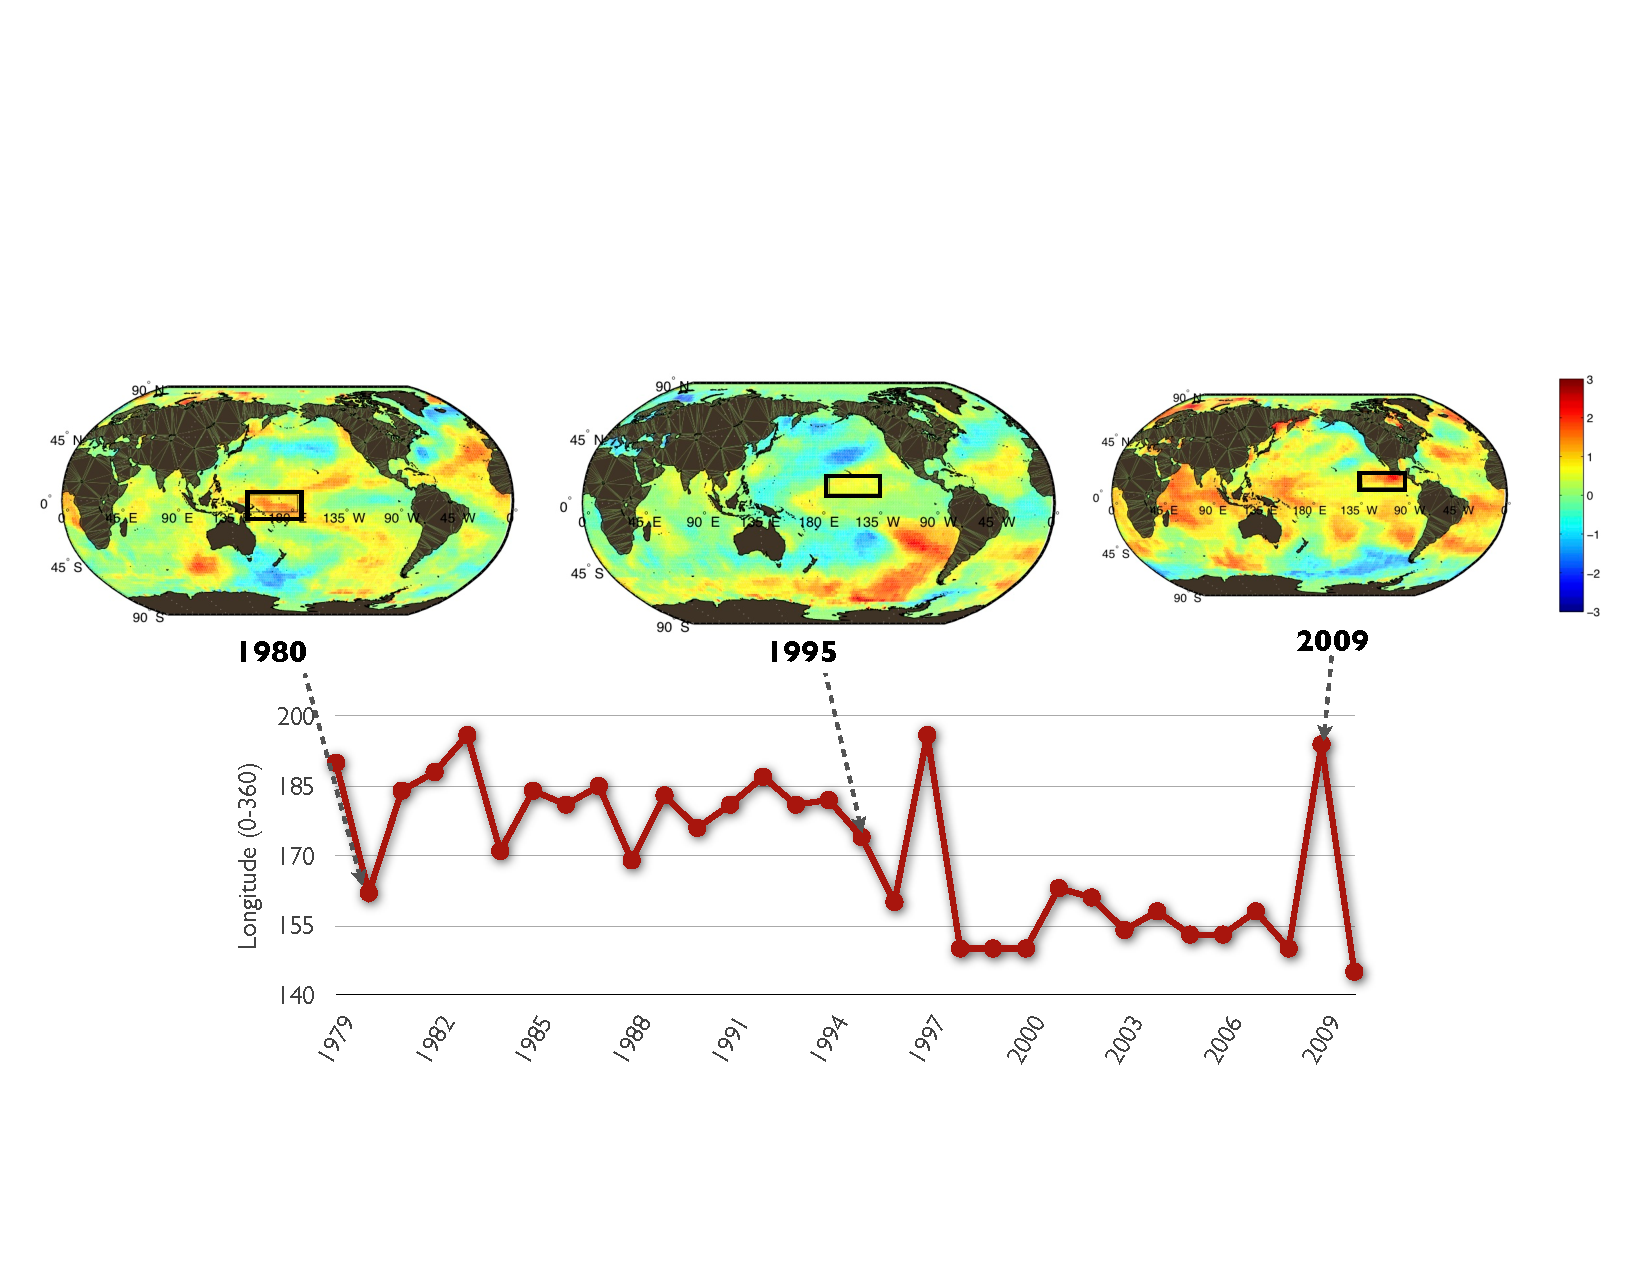
\includegraphics[width=5in]{figures/s_enso_graphic.pdf}
	\caption{A schematic demonstrating how the S-ENSO index is built. First, SST anomalies over a certain month range are computed resulting in maps similar to those above. Next, we search the tropical Pacific for the region with the highest mean SST warming anomaly. Finally, we record the longitude of that region. We repeat this procedure for all years from 1979-2010. }
	\label{fig:s_enso_graphic}
\end{figure}

\subsection{Lead Times Analysis}
For the lead time analysis we tested the robustness of each index, by computing all possible indices as a function of the start and end months of the SST anomalies used to calculate the index. See Figure \ref{fig:figures_monthly_cc_matix}.

We built similar tables as in Figure \ref{fig:figures_monthly_cc_matix} for all the NINO indices. To test the relative robustness of each index to the ENSO spring predictability barrier, we average the performance of each index up to a given month (lead month). To do so, we average all the rows under each end month column. For example, S-ENSO had a mean correlation with Aug-Oct TCs of 0.61 for a July lead. This was obtained by averaging all the rows under July end month in Figure \ref{fig:figures_monthly_cc_matix}. The mean correlation of 0.61 means that if we knew all SST anomalies up to July we could on average explain ~$36\%$ of Aug-Oct variance.

%Figure \ref{fig:figures_lead_time_bar} shows the relative ability of each index to forecast Atlantic TC activity as a function of lead time. Each index (S-ENSO, NINO1.2, \emph{etc.}) is computed by first averaging SST anomalies over a certain month range denoted by a start and end month. The resulting index is then correlated with August-October Atlantic TC counts. For each month on the x-axis, we average the performance of all variations of the indices that end in the month indicated on the chart (end month varies from January to October). 
%For example, the first set of bars were obtained by averaging the performance of all indices end month was January. In this case, there is only one such index the January-January index. The values for the June lead month (number 6 on the x-axis) were obtained by averaging the performance of all indices that had a June end month. There are 6 such indices: January-June, February-June, March-June, April-June, May-June, and June-June. This procedure was repeated for all indices and end months ranging from January to October.

\begin{figure}[htbp]
	\centering
		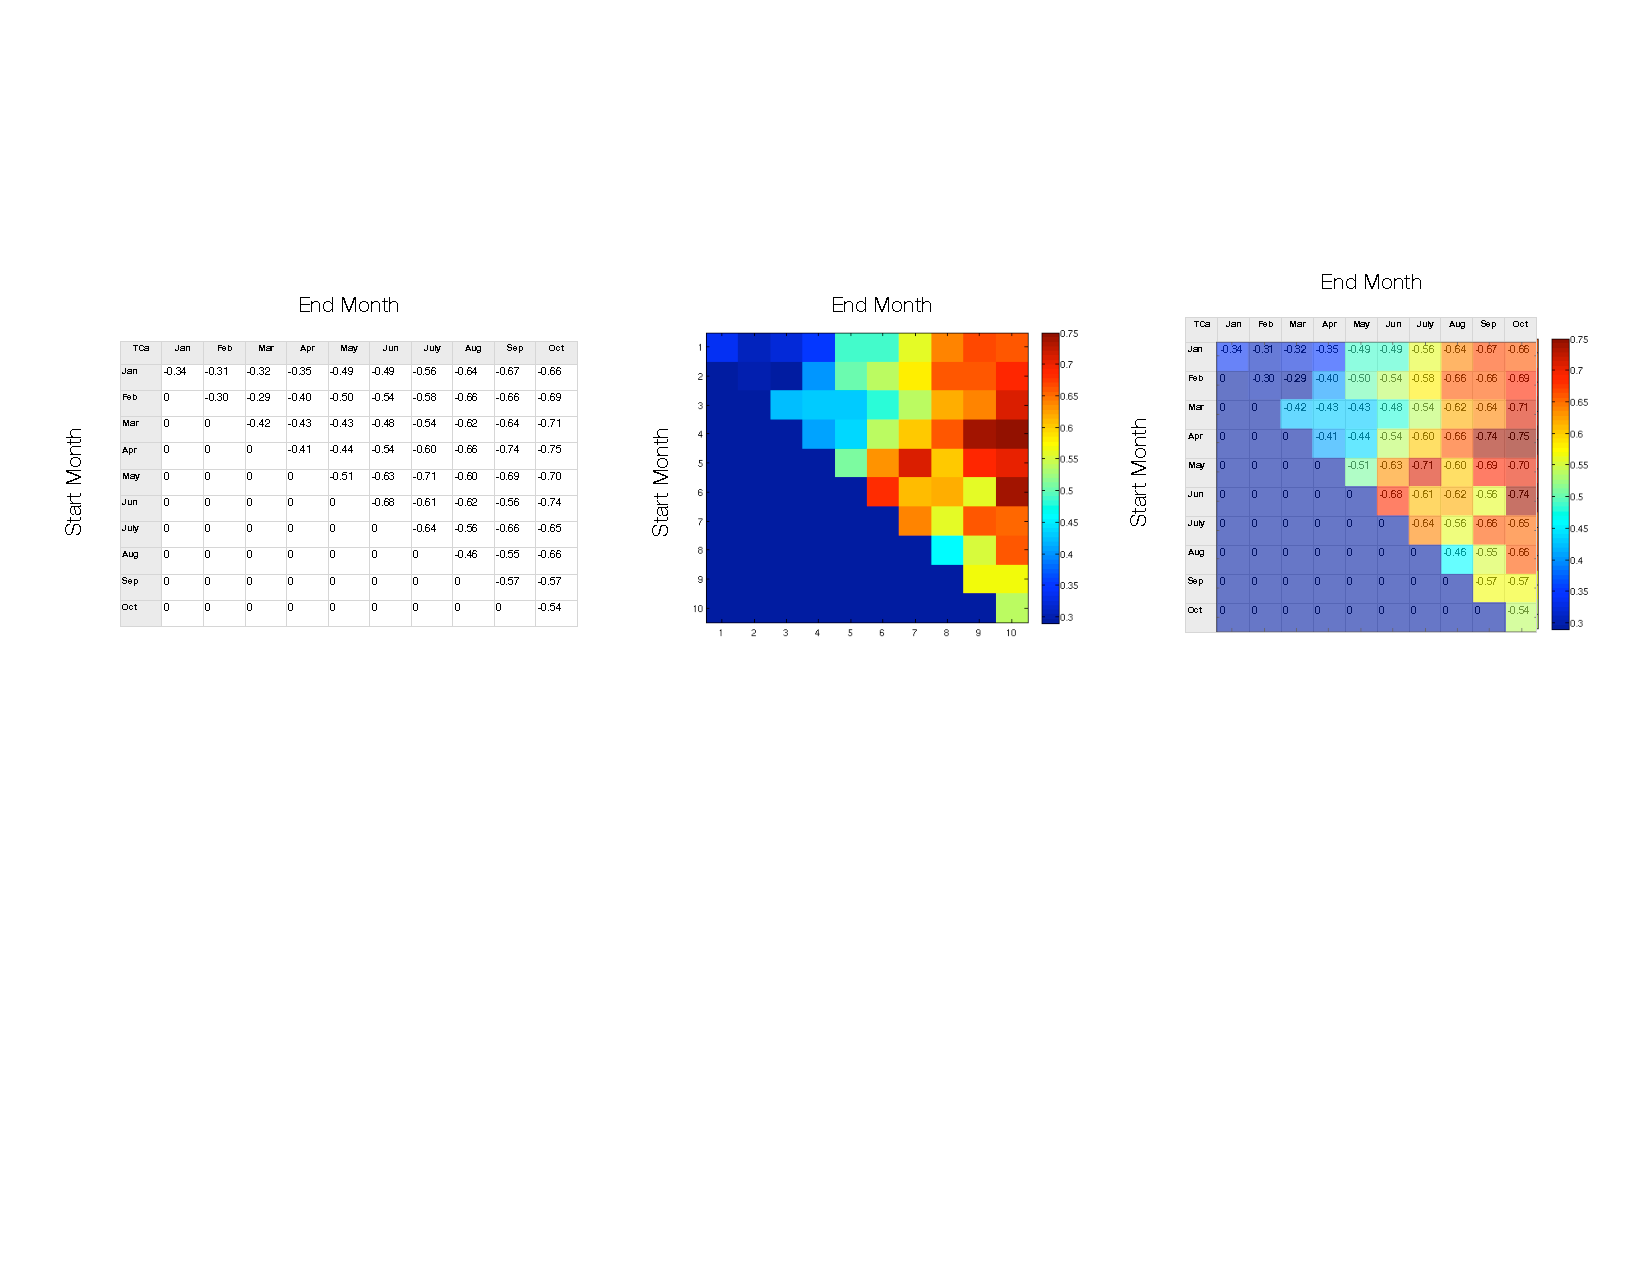
\includegraphics[width=6in]{figures/monthly_cc_matix.pdf}
	\caption{The linear correlation coefficient of every possible S-ENSO index obtained by first averaging SST month anomalies between Start Month (rows) and End Month (columns). S-ENSO's performance increases as the index includes SST anomalies during the Atlantic TC season (June-October).}
	\label{fig:figures_monthly_cc_matix}
\end{figure}



%\subsection{Large-scale composites}
%To compare the large-scale conditions over the Atlantic during active and inactive TC seasons we compute the composites of potential intensity (PI) , saturation deficit, and vertical wind shear -- all elements critical for TC activity. 


\newpage
